\chapter{Module configuration}
This section is intended to provide guidelines for RTA-SUM SOH configuration.

\section {Configuration Parameters}
\subsection {SOHGeneral}
\label{subsection:sohGeneral}

\begin{figure}[H]
	\centering
	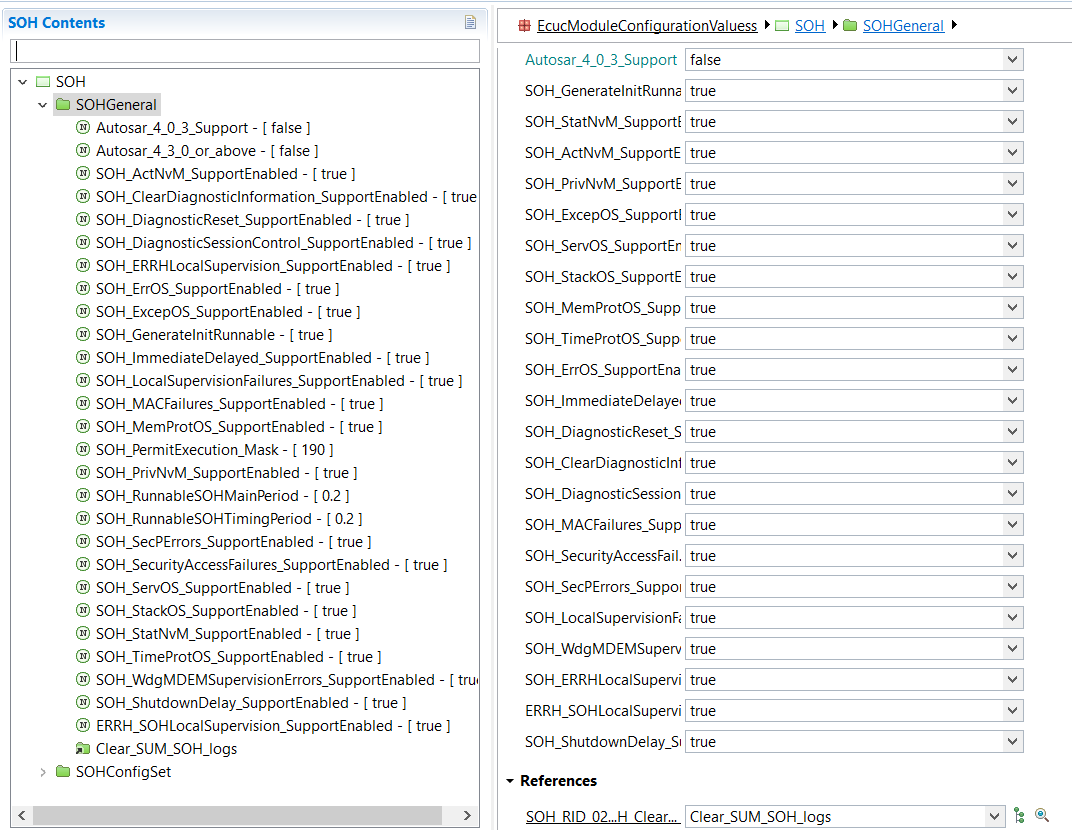
\includegraphics[width=0.8\textwidth]{images/SOHGeneral}
	\caption{SOHGeneral container}
	\label{fig:SOHGeneral}
\end{figure}

\textbf{SOH\_PermitExecution\_Mask}\newline
Mask that can be OR'd with the value supplied by PermitExecution to set any "don't care" bits to '1'.

\textbf{SOH\_RunnableSOHMainPeriod}\newline
This parameter specifies the period (in seconds) of the Runnable\_SOH\_Main, the one that implements the FSM of the module.

\textbf{SohGenerateInitRunnable}\newline
This parameter is used to generate a periodic runnable entity to call SOH\_init function only once.

\textbf{SohInitFuncPeriodicity }\newline
This parameter specifies the time in milisecond for the periodicity of the runnable Runnable\_SOH\_Init.

\textbf{SOH\_StatNvM\_SupportEnabled }\newline
This parameter is used to enable the Nvm Status Failure/Integrity Error class and the relative detector.

\textbf{SOH\_ActNvM\_SupportEnabled }\newline
This parameter is used to enable the Nvm Action Failure Error class and the relative detector.

\textbf{SOH\_ExcepOS\_SupportEnabled}\newline
This parameter is used to enable the OS Hardware Protection Error class and the relative detector.

\textbf{SOH\_ServOS\_SupportEnabled}\newline
This parameter is used to enable the OS Service Protection / Trusted Function Error class and the relative detector.

\textbf{SOH\_StackOS\_SupportEnabled}\newline
This parameter is used to enable the OS Stack Fault class and the relative detector.

\textbf{SOH\_MemProtOS\_SupportEnabled}\newline
This parameter is used to enable the OS Memory Protection Failure Error class and the relative detector.

\textbf{SOH\_TimeProtOS\_SupportEnabled}\newline
This parameter is used to enable the OS Time Protection Error class and the relative detector.

\textbf{SOH\_ErrOS\_SupportEnabled}\newline
This parameter is used to enable the OS Other OS Errors Error class and the relative detector.

\textbf{SOH\_PrivNvM\_SupportEnabled }\newline
This parameter is used to enable the Nvm Privilege class and the relative detector.

\textbf{SOH\_RID\_02C0\_SOH\_Clear\_Log\_Reference}
Reference to DCM RID 0x02C0 SOH Clear Logs 

\textbf{SOH\_ImmediateDelayed\_SupportEnabled}\newline
It allows to enable (disable) for Immediate Reset Detector and Delayed Reset Detector in Reset Reliability monitor.

\textbf{SOH\_DiagnosticReset\_SupportEnabled}\newline
It allows to enable (disable) for Diagnostic Reset Detector in Reset Reliability monitor. 

\textbf{SOH\_ClearDiagnosticInformation\_SupportEnabled}\newline
It allows to enable (disable) for Clear Diagnostic Information Accepted Request Detector and Clear Diagnostic Information Rejected Request Detector in Communication Reliability Monitor.

\textbf{SOH\_DiagnosticSessionControl\_SupportEnabled}\newline
It allows to enable (disable) for Diagnostic Session Control Request Detector and Accepted Diagnostic Session Control Request Detector in Communication Reliability Monitor.

\textbf{SOH\_SecurityAccessFailures\_SupportEnabled}\newline
It allows to enable (disable) for SecurityAccess (Service 0x27) Failures Detector in Communication Reliability Monitor.

\textbf{SOH\_MACFailures\_SupportEnabled}\newline
It allows to enable (disable) for MAC Failures Types 1 and 2 Detector and MAC Failures Type 3 Detector in Communication Reliability Monitor.

\textbf{SOH\_MACFailures\_SupportEnabled}\newline
It allows to enable (disable) for SecP Errors Detector in Communication Reliability Monitor.

\textbf{SOH\_LocalSupervisionFailures\_SupportEnabled}\newline
It allows to enable (disable) for Local Supervision Failures Detector in Watchdog Manager Reliability Monitor.

\textbf{SOH\_WdgMDEMSupervisionErrors\_SupportEnabled}\newline
It allows to enable (disable) for WdgM DEM Supervision Errors Detector in Watchdog Manager Reliability Monitor.

\textbf{SOH\_ERRHLocalSupervision\_SupportEnabled}\newline
It allows to enable (disable) for SUM\_ERRH Local Supervision Detector in Watchdog Manager Reliability Monitor.

\textbf{ERRH\_SOHLocalSupervision\_SupportEnabled}\newline
It allows to enable (disable) for SUM\_SOH Local Supervision Detector implemented by SUM\_ERRH.

\textbf{SOH\_ShutdownDelay\_SupportEnabled}\newline
It allows to enable (disable) for Shutdown Delay Detector in Platform Reliability Monitor.

\textbf{SOH\_RunnableSOHTimingPeriod}\newline
This parameter specifies the period (in seconds) of the runnable Runnable\_SOH\_Timing which implements the time manager for the Time Window Filter and the Shutdown Delay Detector. 

\subsection {SOHConfigSet}
\label{subsection:configset}

\begin{figure}[H]
	\centering
	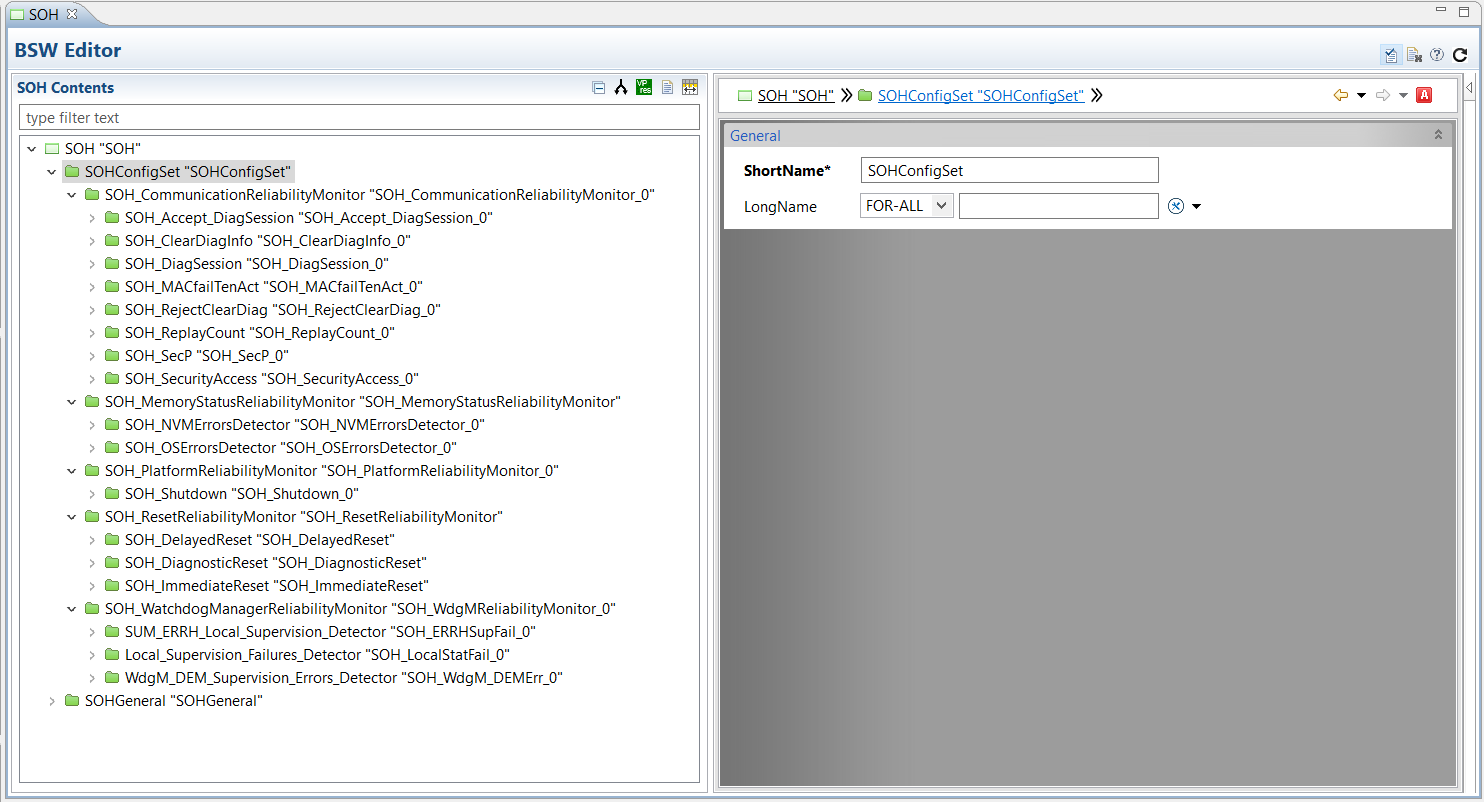
\includegraphics[width=0.85\textwidth]{images/SOHConfigSet}
	\caption{SOHConfigSet container}
	\label{fig:SOHConfigSet}
\end{figure}

\subsubsection{\textbf{SOH\_ResetReliabilityMonitor}}

\textbf{\underline{SOH\_ImmediateReset}}\newline
\textbf{SUM\_SOH\_ImmeReset\_Thresh\_Init}\newline
This parameter specifies the initial value of SUM\_SOH\_ImmeReset\_Thresh

\textbf{SUM\_SOH\_ImmeReset\_TW\_Thresh\_Init}\newline
This parameter specifies the initial value of SUM\_SOH\_ImmeReset\_TW\_Thresh

\textbf{SOH\_NvMImmResetDID\_Reference}\newline
Reference to the NVM DID Block

\textbf{SOH\_DID\_F08F\_ImmResetData\_Reference}\newline
Reference to DCM ImmReset Data

\textbf{\underline{SOH\_DelayedReset}}\newline
\textbf{SUM\_SOH\_DelayedReset\_Thresh\_Init}\newline
This parameter specifies the initial value of SUM\_SOH\_DelayedReset\_Thresh

\textbf{SUM\_SOH\_DelayedReset\_TW\_Thresh\_Init}\newline
This parameter specifies the initial value of SUM\_SOH\_DelayedReset\_TW\_Thresh

\textbf{SOH\_NvMDelayedResetDID\_Reference}\newline
Reference to the NVM DID Block

\textbf{SOH\_DID\_F08F\_DelayedResetData\_Reference}\newline
Reference to DCM DelayedReset Data

\textbf{\underline{SOH\_DiagnosticReset}}\newline
\textbf{SUM\_SOH\_DiagReset\_Thresh\_Init}\newline
This parameter specifies the initial value SUM\_SOH\_DiagReset\_Thresh

\textbf{SOH\_NvMDiagResetCntr\_Reference}\newline
Reference to the NVM Counter Block

\textbf{SOH\_NvMDiagResetDID\_Reference }\newline
Reference to the NVM DID Block

\textbf{SOH\_DID\_F08F\_DiagResetData\_Reference}\newline
Reference to DCM DiagReset Data


\subsubsection{SOH\_CommunicationReliabilityMonitor}

\textbf{\underline{SOH\_ClearDiagInfo}}\newline
\textbf{SUM\_SOH\_ClearDiagInfo\_Thresh\_Init}\newline
This parameter specifies the initial value of SUM\_SOH\_ClearDiagInfo\_Thresh

\textbf{SOH\_NvMClearDiagInfoDID\_Reference}\newline
Reference to the NVM DID Block

\textbf{SOH\_DID\_F092\_ClearDiagInfoDID\_Reference}\newline
Reference to DCM Clear Diag Infomation Data

\textbf{\underline{SOH\_Reject\_ClearDiag}}\newline
\textbf{SUM\_SOH\_Reject\_ClearDiag\_Thresh\_Init}\newline
This parameter specifies the initial value of SUM\_SOH\_Reject\_ClearDiag\_Thresh

\textbf{SOH\_NvMRejectClearDiagDID\_Reference}\newline
Reference to the NVM DID Block

\textbf{SOH\_DID\_F092\_RejectClearDiagDID\_Reference}\newline
Reference to DCM Reject Clear Diag Data

\textbf{\underline{SOH\_Accept\_DiagSession}}\newline
\textbf{SUM\_SOH\_Accept\_DiagSession\_Thresh\_Init}\newline
This parameter specifies the initial value of SUM\_SOH\_Accept\_DiagSession\_Thresh

\textbf{SOH\_NvMAccept\_DiagSessionDID\_Reference}\newline
Reference to the NVM DID Block

\textbf{SOH\_NvMAccept\_DiagSessionCntr\_Reference}\newline
Reference to the NVM DID Block

\textbf{SOH\_DID\_F092\_Accept\_DiagSessionDID\_Reference}\newline
Reference to DCM Accept Diag Session Data

\textbf{\underline{SOH\_DiagSession}}\newline
\textbf{SUM\_SOH\_DiagSession\_Thresh\_Init}\newline
This parameter specifies the initial value of SUM\_SOH\_DiagSession\_Thresh

\textbf{SOH\_NvMDiagSessionDID\_Reference}\newline
Reference to the NVM DID Block

\textbf{SOH\_NvMDiagSessionCntr\_Reference}\newline
Reference to the NVM DID Block

\textbf{SOH\_DID\_F092\_DiagSessionDID\_Reference}\newline
Reference to DCM Diag Session Data

\textbf{\underline{SOH\_SecurityAccess}}\newline
\textbf{SUM\_SOH\_SecurityAccess\_Thresh\_Init}\newline
This parameter specifies the initial value of SUM\_SOH\_SecurityAccess\_Thresh

\textbf{SOH\_NvMSecurityAccessDID\_Reference}\newline
Reference to the NVM DID Block

\textbf{SOH\_NvMSecurityAccessCntr\_Reference}\newline
Reference to the NVM DID Block

\textbf{SOH\_DID\_F092\_SecurityAccessDID\_Reference}\newline
Reference to DCM Security Access Data

\textbf{\underline{SOH\_MACfailTenAct}}\newline
\textbf{SUM\_SOH\_MACfail\_TenAct\_Thresh\_Init}\newline
This parameter specifies the initial value of SUM\_SOH\_MACfail\_TenAct\_Thresh

\textbf{SUM\_SOH\_MACfail\_TenAct\_TW\_Thresh\_Init}\newline
This parameter specifies the initial value of SUM\_SOH\_MACfail\_TenAct\_TW\_Thresh

\textbf{SOH\_NvMMACfail\_TenActDID\_Reference}\newline
Reference to the NVM DID Block

\textbf{SOH\_DID\_F092\_MACfail\_TenActDID\_Reference}\newline
Reference to DCM MAC fail type 1 and 2 Data

\textbf{\underline{SOH\_ReplayCount}}\newline
\textbf{SUM\_SOH\_ReplayCount\_Thresh\_Init}\newline
This parameter specifies the initial value of SUM\_SOH\_ReplayCount\_Thresh

\textbf{SUM\_SOH\_ReplayCount\_TW\_Thresh\_Init}\newline
This parameter specifies the initial value of SUM\_SOH\_ReplayCount\_TW\_Thresh

\textbf{SUM\_SOH\_ReplayCount\_Start\_Thresh\_Init}\newline
This parameter specifies the initial value of SUM\_SOH\_ReplayCount\_Start\_Thresh

\textbf{SOH\_NvMReplayCountDID\_Reference}\newline
Reference to the NVM DID Block

\textbf{SOH\_DID\_F092\_ReplayCountDID\_Reference}\newline
Reference to DCM MAC fail type 3 Data

\textbf{\underline{SOH\_SecP}}\newline
\textbf{SUM\_SOH\_SecP\_Thresh\_Init}\newline
This parameter specifies the initial value of SUM\_SOH\_SecP\_Thresh

\textbf{SUM\_SOH\_SecP\_TW\_Thresh\_Init}\newline
This parameter specifies the initial value of SUM\_SOH\_SecP\_TW\_Thresh

\textbf{SOH\_NvMSecPDID\_Reference}\newline
Reference to the NVM DID Block

\textbf{SOH\_DID\_F092\_SecPDID\_Reference}\newline
Reference to DCM SecP Data

\subsubsection{\textbf{SOH\_MemoryStatusReliabilityMonitor}}
\subsubsection{SOH\_NVMErrorsDetector}
\textbf{\underline{SOH\_StatusNVM}}\newline
\textbf{SUM\_SOH\_StatNVM\_Thresh\_Init}\newline
This parameter specifies the initial value of SUM\_SOH\_StatNVM\_Thresh


\textbf{SUM\_SOH\_StatNVM\_TW\_Thresh\_Init}\newline
This parameter specifies the initial value of SUM\_SOH\_StatNVM\_TW\_Thresh


\textbf{SOH\_NvMActNVMDID\_Reference}\newline
Reference to the NVM DID Block

\textbf{SOH\_DID\_F090\_StatNVM\_Reference}\newline
Reference to DCM StatNVM Data

\textbf{\underline{SOH\_ActNVM}}\newline
\textbf{SUM\_SOH\_ActNVM\_Thresh\_Init}\newline
This parameter specifies the initial value of SUM\_SOH\_ActNVM\_Thresh


\textbf{SUM\_SOH\_ActNVM\_TW\_Thresh\_Init}\newline
This parameter specifies the initial value of SUM\_SOH\_ActNVM\_TW\_Thresh


\textbf{SOH\_NvMActNVMDID\_Reference}\newline
Reference to the NVM DID Block

\textbf{SOH\_DID\_F090\_ActNVM\_Reference}\newline
Reference to DCM ActNVM Data

\textbf{\underline{SOH\_PrivNVM}}\newline
\textbf{SUM\_SOH\_PrivNVM\_Thresh\_Init}\newline
This parameter specifies the initial value of SUM\_SOH\_PrivNVM\_Thresh


\textbf{SUM\_SOH\_PrivNVM\_TW\_Thresh\_Init}\newline
This parameter specifies the initial value of SUM\_SOH\_PrivNVM\_TW\_Thresh


\textbf{SOH\_NvMPrivNVMDID\_Reference}\newline
Reference to the NVM DID Block

\textbf{SOH\_DID\_F090\_PrivNVM\_Reference}\newline
Reference to DCM PrivNVM Data

\subsubsection{SOH\_OSErrorsDetector}
\textbf{\underline{SOH\_ExcepOS}}\newline

\textbf{SUM\_SOH\_ExcepOS\_Thresh\_Init}\newline
Initial value of SUM\_SOH\_ExcepOS\_Thresh

\textbf{SUM\_SOH\_ExcepOS\_TW\_Thresh\_Init}\newline
Initial value of SUM\_SOH\_ExcepOS\_TW\_Thresh

\textbf{SOH\_NvMExcepOSDID\_Reference}\newline
Reference to the NVM DID Block

\textbf{SOH\_DID\_F090\_ExcepOS\_Reference}\newline
Reference to DCM ExcepOS Data

\textbf{\underline{SOH\_ServOS}}\newline


\textbf{SUM\_SOH\_ServOS\_Thresh\_Init}\newline
Initial value of SUM\_SOH\_ServOS\_Thresh

\textbf{SUM\_SOH\_ServOS\_TW\_Thresh\_Init}\newline
Initial value of SUM\_SOH\_ServOS\_TW\_Thresh

\textbf{SOH\_NvMServOSDID\_Reference}\newline
Reference to the NVM DID Block

\textbf{SOH\_DID\_F090\_ServOS\_Reference}\newline
Reference to DCM ServOS Data

\textbf{\underline{SOH\_StackOS}}\newline

\textbf{SUM\_SOH\_StackOS\_Thresh\_Init}\newline
Initial value of SUM\_SOH\_StackOS\_Thresh

\textbf{SUM\_SOH\_StackOS\_TW\_Thresh\_Init}\newline
Initial value of SUM\_SOH\_StackOS\_TW\_Thresh

\textbf{SOH\_NvMServOSDID\_Reference}\newline
Reference to the NVM DID Block

\textbf{SOH\_DID\_F090\_StackOS\_Reference}\newline
Reference to DCM StackOS Data

\textbf{\underline{SOH\_MemProtOS}}\newline

\textbf{SUM\_SOH\_MemProtOS\_Thresh\_Init}\newline
Initial value of SUM\_SOH\_MemProtOS\_Thresh

\textbf{SUM\_SOH\_MemProtOS\_TW\_Thresh\_Init}\newline
Initial value of SUM\_SOH\_MemProtOS\_TW\_Thresh

\textbf{SOH\_NvMMemProtOSDID\_Reference}\newline
Reference to the NVM DID Block

\textbf{SOH\_DID\_F090\_MemProtOS\_Reference}\newline
Reference to DCM MemProtOS Data

\textbf{\underline{SOH\_TimeProtOS}}\newline

\textbf{SUM\_SOH\_TimeProtOS\_Thresh\_Init}\newline
Initial value of SUM\_SOH\_TimeProtOS\_Thresh

\textbf{SUM\_SOH\_TimeProtOS\_TW\_Thresh\_Init}\newline
Initial value of SUM\_SOH\_TimeProtOS\_TW\_Thresh

\textbf{SOH\_NvMTimeProtOSDID\_Reference}\newline
Reference to the NVM DID Block

\textbf{SOH\_DID\_F090\_TimeProtOS\_Reference}\newline
Reference to DCM TimeProtOS Data

\textbf{\underline{SOH\_ErrOS}}\newline

\textbf{SUM\_SOH\_ErrOS\_Thresh\_Init}\newline
Initial value of SUM\_SOH\_ErrOS\_Thresh

\textbf{SUM\_SOH\_ErrOS\_TW\_Thresh\_Init}\newline
Initial value of SUM\_SOH\_ErrOS\_TW\_Thresh

\textbf{SOH\_NvMErrOSDID\_Reference}\newline
Reference to the NVM DID Block

\textbf{SOH\_DID\_F090\_ErrOS\_Reference}\newline
Reference to DCM ErrOS Data

\subsubsection{SOH\_WatchdogManagerReliabilityMonitor}

\textbf{\underline{Local\_Supervision\_Failures\_Detector}}\newline
\textbf{SUM\_SOH\_LocalStatFail\_Thresh\_Init}\newline
This parameter specifies the initial value of SUM\_SOH\_LocalStatFail\_Thresh

\textbf{SUM\_SOH\_LocalStatFail\_TW\_Thresh\_Init}\newline
This parameter specifies the initial value of SUM\_SOH\_LocalStatFail\_TW\_Thresh

\textbf{Supervised\_Entity\_Reference}\newline
This is a reference to a Supervised Entity container in the WdgM. The multiplicity is infinite. All the supervised entities (except the ones
related to ERRH and SOH) should be referenced by using this parameter.

\textbf{SOH\_LocalSupervisionFailures\_DID\_counter\_Reference }\newline
Reference to the NVM Block related to SUM\_SOH\_DID\_LocalStatFail\_Cntr

\textbf{SOH\_DID\_F093\_LocalStatFail\_Reference}\newline
Reference to DCM LocalStatFail Data

\textbf{\underline{WdgM\_DEM\_Supervision\_Errors\_Detector}}\newline
\textbf{SUM\_SOH\_WdgM\_DEMErr\_Thresh\_Init}\newline
This parameter specifies the initial value of SUM\_SOH\_WdgM\_DEMErr\_Thresh

\textbf{SUM\_SOH\_WdgM\_DEMErr\_TW\_Thresh\_Init}\newline
This parameter specifies the initial value of SUM\_SOH\_WdgM\_DEMErr\_TW\_Thresh

\textbf{SOH\_WdgMDEMErr\_DID\_counter\_Reference}\newline
Reference to the NVM Block related to SUM\_SOH\_DID\_WdgM\_DEMErr\_Cntr

\textbf{SOH\_DID\_F093\_WdgMDEMErr\_Reference}\newline
Reference to DCM WdgMDEMErr Data

\textbf{\underline{SUM\_ERRH\_Local\_Supervision\_Detector}}\newline
\textbf{SOH\_ERRHSupFail\_Thresh\_Init}\newline
This parameter specifies the initial value of SOH\_ERRHSupFail\_Thresh

\textbf{SOH\_ERRHSupFail\_TW\_Thresh\_Init}\newline
This parameter specifies the initial value of SOH\_ERRHSupFail\_TW\_Thresh

\textbf{SOH\_ERRHLocalSupervisionFailures\_DID\_counter\_Reference}\newline
Reference to the NVM Block related to SUM\_SOH\_DID\_ERRHSupFail\_Cntr

\textbf{SOH\_DID\_F093\_ERRHSupFail\_Reference}\newline
Reference to DCM ERRHSupFail Data

\textbf{SOH\_DID\_F093\_ERRH\_Local\_Supervision\_Status\_Reference}\newline
Reference to DCM ERRH Local Supervision Status Data

\subsubsection{SOH\_PlatformReliabilityMonitor}

\textbf{\underline{SOH\_Shutdown}}\newline
\textbf{SUM\_SOH\_Shutdown\_Thresh\_Init}\newline
This parameter specifies the initial value of SUM\_SOH\_Shutdown\_Thresh

\textbf{SUM\_SOH\_ShutDown\_Timer\_Thresh\_Init}\newline
This parameter specifies the initial value of SUM\_SOH\_ShutDown\_Timer\_Thresh

\textbf{SOH\_NvMShutdownDID\_Reference}\newline
Reference to the NVM DID Block

\textbf{SOH\_NvMShutdownCntr\_Reference}\newline
Reference to the NVM Counter Block

\textbf{SOH\_DID\_F091\_ShutdownDID\_Reference}\newline
Reference to DCM Shutdown DID counter Data


\section{Configuration Hints}
\subsection{SOH Initialization}
\label{subsec:SohInit}
To correctly initialize the module, the user can follow two possible paths depending on the configured value for the boolean parameter \code{SohGenerateInitRunnable} :
\begin{itemize}
\item If it is false, the user shall invoke the SUM\_SOH initialization function \code{SOH_Init()}, which is an external function declared in the header file \file{SUM_SOH.h}. The BswM should invoke this function at initialization time through a BswMAction.
\item If it is true, the user shall configure the \code{SohInitFuncPeriodicity} parameter, which specifies the periodicity of the \code{Runnable_SOH_Init} in ms, and schedule the init runnable in a lower periodicity OS task.
	  In this case, a periodic runnable is generated to execute the internal \code{SOH_Init()} function.
\end{itemize}

\subsection{Memory Types}
\label{subsec:memory}
SUM\_SOH requires four different types of memory : 

\begin{itemize}
	\item RAM
	\item Non Cleared RAM
    \item Adaptable NVM
    \item Secure Cumulative NVM
\end{itemize}


The ECU shall have a NvM Module fulfilling the requirements for Adaptable NVM and Secure Cumulative NVM definitions.

One Block for each NvM metric shall be created (30 different blocks), each block shall fulfill the respective requirements for Adaptable NVM or Secure Cumulative NVM definitions.

Each NvM block shall have the \textbf{NvMRamBlockDataAddress} set to the relative RTE generated ArPim variable like in the figure \ref{fig:NvM}
\begin{figure}[H]
\centering
	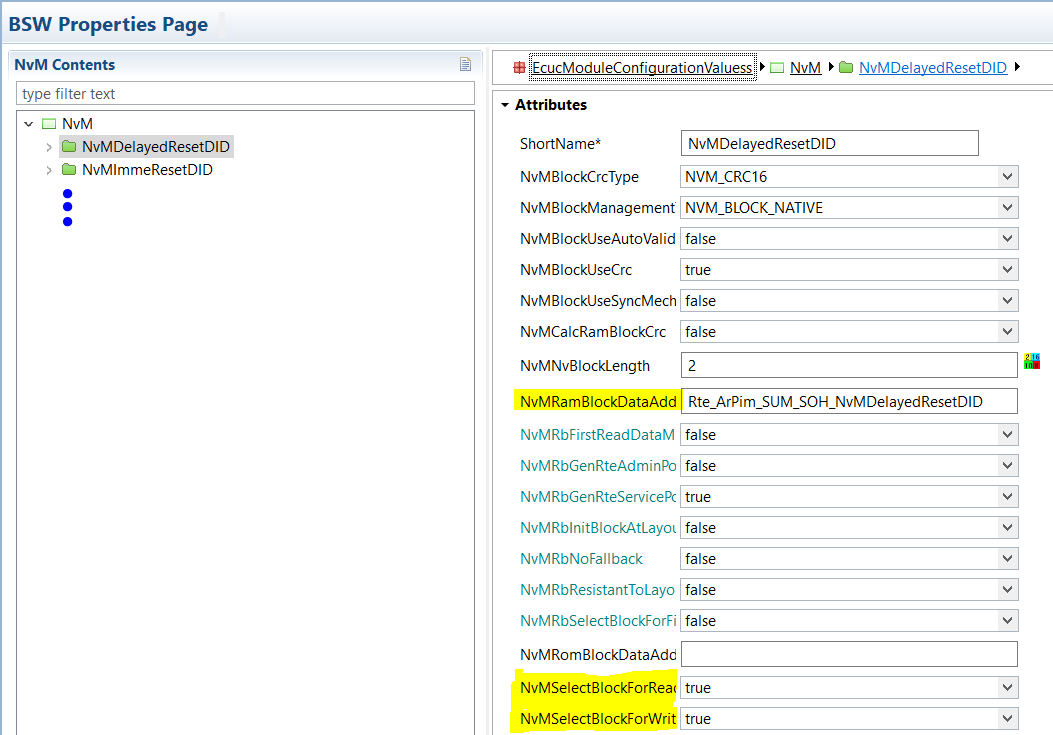
\includegraphics[scale=0.6]{images/NvM}
	\caption{example of NvM block}
	\label{fig:NvM}
\end{figure}

For RAM and Non Cleared RAM types, the user shall use the MemMapGen generator to generate the \code{SUM_SOH_MemMap.h} file.
This file will contain the necessary memory sections, defined in the SWCD (Figure: \ref{fig:memsec}), as below:
\begin{itemize}
	\item \code{SUM_SOH_SEC_CODE} used for Code.
    \item \code{SUM_SOH_SEC_VAR_POWER_ON_CLEARED_BOOLEAN} used for Non Cleared RAM boolean.
	\item \code{SUM_SOH_SEC_VAR_POWER_ON_CLEARED_16} used for Non Cleared RAM 16Bit.
	\item \code{SUM_SOH_SEC_VAR_POWER_ON_CLEARED_32} used for Non Cleared RAM 32Bit.
    \item \code{SUM_SOH_SEC_VAR_CLEARED_BOOLEAN} used for all the others boolean.
	\item \code{SUM_SOH_SEC_VAR_CLEARED_16} used for all the others 16Bit.
	\item \code{SUM_SOH_SEC_VAR_CLEARED_32} used for all the others 32Bit.
    \item \code{SUM_SOH_SEC_VAR_CLEARED_UNSPECIFIED} used for structures and array.
\end{itemize}

\begin{figure}[H]
	\centering
	\includegraphics[scale=0.6]{images/Swcd\_memsections.png}
	\caption{Memory sections defined in the SWCD arxml file.}
	\label{fig:memsec}
\end{figure}

\subsection{Main FSM}
The main SOH Finite State Machine is implemented by the Runnable\_SOH\_Main. It manages three states:
\begin{itemize}
    \item SOH\_INIT\_MODE
    \item SOH\_NORMAL\_MODE
    \item SOH\_SHUTDOWN\_MODE
\end{itemize}

To properly work it needs the following port connections :

\begin{itemize}
    \item \code{SUSD_SOH_PermitExecution} with the SUSD
    \item \code{SOH_SUSD_ShutdownPermission} with the SUSD
    \item \code{DIAG_SOH_GetMEC} with the DIAG
\end{itemize}

Also the parameter \code{SOH_RunnableSOHMainPeriod} must be configured with the right periodicity for this runnable and the parameter
\code{SOH_PermitExecution_Mask} with the appropriate byte to process the PermitExecution information outputed by SUSD.


\subsection{Time Manager}
\label{subsec:timeManager}
SUM\_SOH implements a periodic runnable (Runnable\_SOH\_Timing) that calls the OS API GetCounterValue() to read the counter Rte\_TickCounter and pass it to:
\begin{itemize}
	\item the Time Window Filter
	\item the ShutDown Delay Detector.
\end{itemize}

The periodicity of this runnable is configurable through the parameter \\ SOHGeneral/SOH\_RunnableSOHTimingPeriod. \newline

Please note that this periodicity shall be less than 1 second in order to assure the proper increment of the time window timer and the shutdown delay timer.


\subsection{Time Window Filter}
\label{subsec:TimeWindowFilter}
SUM\_SOH needs to update the time windows value when the relative filtering is started. 

The calculation of the elapsed time is based on the ticks of a counter read periodically by the Time Manager Runnable (see \ref{subsec:timeManager}).\\
The difference between the current ticks value and the previous one is converted in seconds: at least 1 second should elapse to increase a time window.\\
The previous value is initialized to 0 and reset to 0 when a new detection cycle starts.\\
If the previous value is 0, the difference is not computed.


\subsection{Reliability Monitor}
\subsubsection{Reset Reliability Monitor}

To integrate the Reset Reliability Monitor you must schedule the following Runnables in a Data Receive Event OS Task :

\begin{itemize}
    \item \code{Runnable_SOHResetReliabilityMonitor_ImmeDelayedReset}
    \item \code{Runnable_SOHResetReliabilityMonitor_DiagReset}
\end{itemize}


Four NvM blocks must be created in the NvM :

\begin{tabular}{|l|p{8cm}|}\hline
\multicolumn{2}{|c|}{\textbf{DID\_ImmeReset}}\\\hline
NvMNvBlockLength&2\\\hline
NvMRamBlockDataAddress&Rte\_ArPim\_SUM\_SOH\_NvMImmeResetDID\\\hline
NvMSelectBlockForReadAll&TRUE\\\hline
NvMSelectBlockForWriteAll&TRUE\\\hline
Configure as&Secure Cumulative NVM\\\hline
\end{tabular}

\begin{tabular}{|l|p{8cm}|}\hline
\multicolumn{2}{|c|}{\textbf{DID\_DelayedReset}}\\\hline
NvMNvBlockLength&2\\\hline
NvMRamBlockDataAddress&Rte\_ArPim\_SUM\_SOH\_NvMDelayedResetDID\\\hline
NvMSelectBlockForReadAll&TRUE\\\hline
NvMSelectBlockForWriteAll&TRUE\\\hline
Configure as&Secure Cumulative NVM\\\hline
\end{tabular}

\begin{tabular}{|l|p{8cm}|}\hline
\multicolumn{2}{|c|}{\textbf{DiagResetCntr}}\\\hline
NvMNvBlockLength&2\\\hline
NvMRamBlockDataAddress&Rte\_ArPim\_SUM\_SOH\_NvMDiagResetCntr\\\hline
NvMSelectBlockForReadAll&TRUE\\\hline
NvMSelectBlockForWriteAll&TRUE\\\hline
Configure as&Adaptable NVM\\\hline
\end{tabular}

\begin{tabular}{|l|p{8cm}|}\hline
\multicolumn{2}{|c|}{\textbf{DID\_DiagResetCntr}}\\\hline
NvMNvBlockLength&2\\\hline
NvMRamBlockDataAddress&Rte\_ArPim\_SUM\_SOH\_NvMDiagResetDID\\\hline
NvMSelectBlockForReadAll&TRUE\\\hline
NvMSelectBlockForWriteAll&TRUE\\\hline
Configure as&Secure Cumulative NVM\\\hline
\end{tabular}


Interfaces that must be connected with the other SUMs :

\begin{itemize}
    \item \code{SUSD_SOH_ResetOccured} with the SUSD relative Port
    \item \code{DIAG_ECUResetRequest} with the DIAG relative Port
    \item \code{NvMService} with the NvM relative Port
\end{itemize}

\subsubsection{Memory Status Reliability Monitor}
\label{subsubsection:msrm}
To integrate the Memory Status Reliability Monitor you must schedule the following Runnable in a Data Receive Event OS Task :

\begin{itemize}
    \item \code{Runnable_SOH_ERRH_BswEvent}
\end{itemize}

And you shall use the following CallBack Function within OS ErrorHook(s):

\begin{itemize}
	\item \code{SOH_OS_Protection_ErrorHook_CallBack}
\end{itemize}

Nine NvM blocks must be created in the NvM :

\begin{tabular}{|l|p{8cm}|}\hline
\multicolumn{2}{|c|}{\textbf{DID\_NvMStat}}\\\hline
NvMNvBlockLength&2\\\hline
NvMRamBlockDataAddress&Rte\_ArPim\_SUM\_SOH\_NvMStatDID\\\hline
NvMSelectBlockForReadAll&TRUE\\\hline
NvMSelectBlockForWriteAll&TRUE\\\hline
Configure as&Secure Cumulative NVM\\\hline
\end{tabular}

\begin{tabular}{|l|p{8cm}|}\hline
\multicolumn{2}{|c|}{\textbf{DID\_NvMAct}}\\\hline
NvMNvBlockLength&2\\\hline
NvMRamBlockDataAddress&Rte\_ArPim\_SUM\_SOH\_NvMActDID\\\hline
NvMSelectBlockForReadAll&TRUE\\\hline
NvMSelectBlockForWriteAll&TRUE\\\hline
Configure as&Secure Cumulative NVM\\\hline
\end{tabular}

\begin{tabular}{|l|p{8cm}|}\hline
\multicolumn{2}{|c|}{\textbf{DID\_NvMPriv}}\\\hline
NvMNvBlockLength&2\\\hline
NvMRamBlockDataAddress&Rte\_ArPim\_SUM\_SOH\_NvMPrivDID\\\hline
NvMSelectBlockForReadAll&TRUE\\\hline
NvMSelectBlockForWriteAll&TRUE\\\hline
Configure as&Secure Cumulative NVM\\\hline
\end{tabular}


\begin{tabular}{|l|p{8cm}|}\hline
\multicolumn{2}{|c|}{\textbf{DID\_ExcepOS}}\\\hline
NvMNvBlockLength&2\\\hline
NvMRamBlockDataAddress&Rte\_ArPim\_SUM\_SOH\_ExcepOSDID\\\hline
NvMSelectBlockForReadAll&TRUE\\\hline
NvMSelectBlockForWriteAll&TRUE\\\hline
Configure as&Secure Cumulative NVM\\\hline
\end{tabular}

\begin{tabular}{|l|p{8cm}|}\hline
\multicolumn{2}{|c|}{\textbf{DID\_ServOS}}\\\hline
NvMNvBlockLength&2\\\hline
NvMRamBlockDataAddress&Rte\_ArPim\_SUM\_SOH\_ServOSDID\\\hline
NvMSelectBlockForReadAll&TRUE\\\hline
NvMSelectBlockForWriteAll&TRUE\\\hline
Configure as&Secure Cumulative NVM\\\hline
\end{tabular}

\begin{tabular}{|l|p{8cm}|}\hline
	\multicolumn{2}{|c|}{\textbf{DID\_StackOS}}\\\hline
	NvMNvBlockLength&2\\\hline
	NvMRamBlockDataAddress&Rte\_ArPim\_SUM\_SOH\_StackOSDID\\\hline
	NvMSelectBlockForReadAll&TRUE\\\hline
	NvMSelectBlockForWriteAll&TRUE\\\hline
	Configure as&Secure Cumulative NVM\\\hline
	\end{tabular}

\begin{tabular}{|l|p{8cm}|}\hline
\multicolumn{2}{|c|}{\textbf{DID\_MemProtOS}}\\\hline
NvMNvBlockLength&2\\\hline
NvMRamBlockDataAddress&Rte\_ArPim\_SUM\_SOH\_MemProtOSDID\\\hline
NvMSelectBlockForReadAll&TRUE\\\hline
NvMSelectBlockForWriteAll&TRUE\\\hline
Configure as&Secure Cumulative NVM\\\hline
\end{tabular}

\begin{tabular}{|l|p{8cm}|}\hline
\multicolumn{2}{|c|}{\textbf{DID\_TimeProtOS}}\\\hline
NvMNvBlockLength&2\\\hline
NvMRamBlockDataAddress&Rte\_ArPim\_SUM\_SOH\_TimeProtOSDID\\\hline
NvMSelectBlockForReadAll&TRUE\\\hline
NvMSelectBlockForWriteAll&TRUE\\\hline
Configure as&Secure Cumulative NVM\\\hline
\end{tabular}

\begin{tabular}{|l|p{8cm}|}\hline
\multicolumn{2}{|c|}{\textbf{DID\_ErrOS}}\\\hline
NvMNvBlockLength&2\\\hline
NvMRamBlockDataAddress&Rte\_ArPim\_SUM\_SOH\_ErrOSDID\\\hline
NvMSelectBlockForReadAll&TRUE\\\hline
NvMSelectBlockForWriteAll&TRUE\\\hline
Configure as&Secure Cumulative NVM\\\hline
\end{tabular}


To enable, disable the relative NvM error class you must configure the following configuration parameters:\newline
\begin{center}\begin{tabular}{|l|c|}
\hline
\textbf{Configuration Parameter}    & \textbf{Detector}               \\ \hline
SOH\_StatNvM\_SupportEnabled      &  Status Failure/Integrity       \\ \hline
SOH\_ActNvM\_SupportEnabled       &  Action Failure                 \\ \hline
SOH\_PrivNvM\_SupportEnabled      &  Privilege                      \\ \hline
\hline
\end{tabular}\end{center}

To enable, disable the relative OS error class you must configure the following configuration parameters:\newline

\begin{center}\begin{tabular}{|l|c|}
\hline
\textbf{Configuration Parameter}    & \textbf{Detector}                       \\ \hline
SOH\_ExcepOS\_SupportEnabled      & Hardware Protection                     \\ \hline
SOH\_ServOS\_SupportEnabled       & Service Protection / Trusted Function   \\ \hline
SOH\_StackOS\_SupportEnabled      & Stack Fault                             \\ \hline
SOH\_MemProtOS\_SupportEnabled    & Memory Protection                       \\ \hline
SOH\_TimeProtOS\_SupportEnabled   & Time Protection                         \\ \hline
SOH\_ErrOS\_SupportEnabled        & Other OS Errors                         \\ \hline
\hline
\end{tabular}\end{center}

Interfaces that must be connected with the other SUMs :

\begin{itemize}
    \item \code{ERRH_E_BswEvent} with the ERRH relative Port
\end{itemize}


\subsubsection{Communication Reliability Monitor}

\paragraph{Event-Triggered Runnables to schedule}
To integrate the Communication Reliability Monitor you must schedule the following Runnables in a Data Receive Event OS Task:

\begin{itemize}
    \item \code{Runnable_SOH_CommunicationReliabilityMonitor_ClearDiag()}
    \item \code{Runnable_SOH_CommunicationReliabilityMonitor_DiagSession()}
    \item \code{Runnable_SOH_CommunicationReliabilityMonitor_AcceptDiagSession()}
    \item \code{Runnable_SOH_CommunicationReliabilityMonitor_SecurityAccess()}
    \item \code{Runnable_SOH_CommunicationReliabilityMonitor_MacFailType123()}
    \item \code{Runnable_SOH_CommunicationReliabilityMonitor_SecP()}
\end{itemize}


\paragraph{Periodic Runnables to schedule}
To integrate the Communication Reliability Monitor you must schedule the following Runnables in a Time Event OS Task:

\begin{itemize}
    \item \code{Runnable_SOH_CommunicationReliabilityMonitor_MacFailType3Delay()}
\end{itemize}


\paragraph{NvM blocks to create}
To integrate the Communication Reliability Monitor you must create the following NvM blocks in the NvM:

\begin{tabular}{|l|p{8cm}|}\hline
\multicolumn{2}{|c|}{\textbf{DID\_ClearDiagInfo}}\\\hline
NvMNvBlockLength&2\\\hline
NvMRamBlockDataAddress&Rte\_ArPim\_SUM\_SOH\_NvMClearDiagInfoDID\\\hline
NvMSelectBlockForReadAll&TRUE\\\hline
NvMSelectBlockForWriteAll&TRUE\\\hline
Configure as&Secure Cumulative NVM\\\hline
\end{tabular}

\begin{tabular}{|l|p{8cm}|}\hline
\multicolumn{2}{|c|}{\textbf{DID\_Reject\_ClearDiag}}\\\hline
NvMNvBlockLength&2\\\hline
NvMRamBlockDataAddress&Rte\_ArPim\_SUM\_SOH\_NvMRejectClearDiagDID\\\hline
NvMSelectBlockForReadAll&TRUE\\\hline
NvMSelectBlockForWriteAll&TRUE\\\hline
Configure as&Secure Cumulative NVM\\\hline
\end{tabular}

\begin{tabular}{|l|p{8cm}|}\hline
\multicolumn{2}{|c|}{\textbf{DID\_DiagSession}}\\\hline
NvMNvBlockLength&2\\\hline
NvMRamBlockDataAddress&Rte\_ArPim\_SUM\_SOH\_NvMDiagSessionDID\\\hline
NvMSelectBlockForReadAll&TRUE\\\hline
NvMSelectBlockForWriteAll&TRUE\\\hline
Configure as&Secure Cumulative NVM\\\hline
\end{tabular}

\begin{tabular}{|l|p{8cm}|}\hline
\multicolumn{2}{|c|}{\textbf{DID\_Accept\_DiagSession}}\\\hline
NvMNvBlockLength&2\\\hline
NvMRamBlockDataAddress&Rte\_ArPim\_SUM\_SOH\_NvMAcceptDiagSessionDID\\\hline
NvMSelectBlockForReadAll&TRUE\\\hline
NvMSelectBlockForWriteAll&TRUE\\\hline
Configure as&Secure Cumulative NVM\\\hline
\end{tabular}

\begin{tabular}{|l|p{8cm}|}\hline
\multicolumn{2}{|c|}{\textbf{DID\_SecurityAccess}}\\\hline
NvMNvBlockLength&2\\\hline
NvMRamBlockDataAddress&Rte\_ArPim\_SUM\_SOH\_NvMSecurityAccessDID\\\hline
NvMSelectBlockForReadAll&TRUE\\\hline
NvMSelectBlockForWriteAll&TRUE\\\hline
Configure as&Secure Cumulative NVM\\\hline
\end{tabular}

\begin{tabular}{|l|p{8cm}|}\hline
\multicolumn{2}{|c|}{\textbf{DID\_MACfail\_TenAct}}\\\hline
NvMNvBlockLength&2\\\hline
NvMRamBlockDataAddress&Rte\_ArPim\_SUM\_SOH\_NvMMACfailTenActDID\\\hline
NvMSelectBlockForReadAll&TRUE\\\hline
NvMSelectBlockForWriteAll&TRUE\\\hline
Configure as&Secure Cumulative NVM\\\hline
\end{tabular}

\begin{tabular}{|l|p{8cm}|}\hline
\multicolumn{2}{|c|}{\textbf{DID\_ReplayCount}}\\\hline
NvMNvBlockLength&2\\\hline
NvMRamBlockDataAddress&Rte\_ArPim\_SUM\_SOH\_NvMReplayCountDID\\\hline
NvMSelectBlockForReadAll&TRUE\\\hline
NvMSelectBlockForWriteAll&TRUE\\\hline
Configure as&Secure Cumulative NVM\\\hline
\end{tabular}

\begin{tabular}{|l|p{8cm}|}\hline
\multicolumn{2}{|c|}{\textbf{DID\_SecP}}\\\hline
NvMNvBlockLength&2\\\hline
NvMRamBlockDataAddress&Rte\_ArPim\_SUM\_SOH\_NvMSecPDID\\\hline
NvMSelectBlockForReadAll&TRUE\\\hline
NvMSelectBlockForWriteAll&TRUE\\\hline
Configure as&Secure Cumulative NVM\\\hline
\end{tabular}

\begin{tabular}{|l|p{8cm}|}\hline
\multicolumn{2}{|c|}{\textbf{DiagSessionCntr}}\\\hline
NvMNvBlockLength&2\\\hline
NvMRamBlockDataAddress&Rte\_ArPim\_SUM\_SOH\_NvMDiagSessionCntr\\\hline
NvMSelectBlockForReadAll&TRUE\\\hline
NvMSelectBlockForWriteAll&TRUE\\\hline
Configure as&Secure Cumulative NVM\\\hline
\end{tabular}

\begin{tabular}{|l|p{8cm}|}\hline
\multicolumn{2}{|c|}{\textbf{Accept\_DiagSessionCntr}}\\\hline
NvMNvBlockLength&2\\\hline
NvMRamBlockDataAddress&Rte\_ArPim\_SUM\_SOH\_NvMAcceptDiagSessionCntr\\\hline
NvMSelectBlockForReadAll&TRUE\\\hline
NvMSelectBlockForWriteAll&TRUE\\\hline
Configure as&Secure Cumulative NVM\\\hline
\end{tabular}

\begin{tabular}{|l|p{8cm}|}\hline
\multicolumn{2}{|c|}{\textbf{SecurityAccessCntr}}\\\hline
NvMNvBlockLength&2\\\hline
NvMRamBlockDataAddress&Rte\_ArPim\_SUM\_SOH\_NvMSecurityAccessCntr\\\hline
NvMSelectBlockForReadAll&TRUE\\\hline
NvMSelectBlockForWriteAll&TRUE\\\hline
Configure as&Secure Cumulative NVM\\\hline
\end{tabular}

\paragraph{Interfaces to connect}
To integrate the Communication Reliability Monitor you must connect the following interfaces with the other SUMs:

\begin{itemize}
    \item \code{SSFM_ClearDiagReq} with the SSFM relative Port
    \item \code{DIAG_SOH_DiagSessionRequest} with the DIAG relative Port
    \item \code{DiagnosticReprogrammingRequest} with the BswM relative Port
    \item \code{SSC_SOH_SecurityAccessError} with the SSC relative Port
    \item \code{SSC_E_SecureMessageMonitoringEvents} with the SSC relative Port
    \item \code{RP_ErrorStatus} with the BswM relative Port
\end{itemize}

\subsubsection{Watchdog Manager Reliability Monitor}

To integrate the Watchdog Manager Reliability Monitor you must schedule the following Runnables in an OS Task :

\begin{itemize}
    \item \code{Runnable_WdgMReliabilityMonitor_FailedLocalSupervision_\<Supervised\_Entity\_name\>}
    \item \code{Runnable_SOH_BswEventsMonitor_NvM_DEM_Errors_Detector}
	\item \code{Runnable_SOH_WdgMReliabilityMonitor_ERRHFailedLocalSupervision}
\end{itemize}


Three NvM block must be created in the NvM :

\begin{tabular}{|l|p{10.5cm}|}\hline
\multicolumn{2}{|c|}{\textbf{NvMBlock\_SOH\_LocalSupervisionFailures\_DID\_counter}}\\\hline
NvMNvBlockLength&2\\\hline
NvMRamBlockDataAddress&Rte\_ArPim\_SUM\_SOH\_LocalSupervisionFailuresDID\_counter\\\hline
NvMSelectBlockForReadAll&TRUE\\\hline
NvMSelectBlockForWriteAll&TRUE\\\hline
Configure as&Secure Cumulative NVM\\\hline
\end{tabular}

\begin{tabular}{|l|p{10.5cm}|}\hline
\multicolumn{2}{|c|}{\textbf{NvMBlock\_SOH\_WdgMDEMErr\_DID\_counter}}\\\hline
NvMNvBlockLength&2\\\hline
NvMRamBlockDataAddress&Rte\_ArPim\_SUM\_SOH\_WdgMDEMErr\_DID\_counter\\\hline
NvMSelectBlockForReadAll&TRUE\\\hline
NvMSelectBlockForWriteAll&TRUE\\\hline
Configure as&Secure Cumulative NVM\\\hline
\end{tabular}

\begin{tabular}{|l|p{10.5cm}|}\hline
\multicolumn{2}{|c|}{\textbf{NvMBlock\_SOH\_ERRHLocalSupervisionFailures\_DID\_counter}}\\\hline
NvMNvBlockLength&2\\\hline
NvMRamBlockDataAddress&Rte\_ArPim\_SUM\_SOH\_ERRHLocalSupervisionFailures\_DID\_counter\\\hline
NvMSelectBlockForReadAll&TRUE\\\hline
NvMSelectBlockForWriteAll&TRUE\\\hline
Configure as&Secure Cumulative NVM\\\hline
\end{tabular}


Interfaces that must be connected with:

\begin{itemize}
    \item \code{SOH\_WdgM\_IndividualMode\<1...n\>} with the WdgM corresponding WdgM \_LocalMode Port interface.
    \item \code{ERRH_E_BswEvent} with the ERRH corresponding Port
	\item \code{SOH_WdgM_IndividualMode_Errh} with the WdgM corresponding WdgM \_LocalMode Port interface.
    \item \code{NvMService} with the NvM corresponding Ports
\end{itemize}

\paragraph{Watchdog Manager Configuration}
Look section \ref{subsection:wdgm} for details.

\subsubsection{Platform Reliability Monitor}
\label{subsec:PlatformReliabilityMonitor}

\paragraph{NvM blocks to create}
To integrate the Platform Reliability Monitor you must create the following NvM blocks in the NvM:

\begin{tabular}{|l|p{8cm}|}\hline
\multicolumn{2}{|c|}{\textbf{ShutDownCntr}}\\\hline
NvMNvBlockLength&2\\\hline
NvMRamBlockDataAddress&Rte\_ArPim\_SUM\_SOH\_NvMShutDownCntr\\\hline
NvMSelectBlockForReadAll&TRUE\\\hline
NvMSelectBlockForWriteAll&TRUE\\\hline
Configure as&Adaptive NVM\\\hline
\end{tabular}

\begin{tabular}{|l|p{8cm}|}\hline
\multicolumn{2}{|c|}{\textbf{DID\_ShutDown}}\\\hline
NvMNvBlockLength&2\\\hline
NvMRamBlockDataAddress&Rte\_ArPim\_SUM\_SOH\_NvMShutDownDID\\\hline
NvMSelectBlockForReadAll&TRUE\\\hline
NvMSelectBlockForWriteAll&TRUE\\\hline
Configure as&Secure Cumulative NVM\\\hline
\end{tabular}

\paragraph{Interfaces to connect}
To integrate the Platform Reliability Monitor you must connect the following interfaces with the other SUMs:

\begin{itemize}
\item \code{PNC_SUSD_ShutdownPermission} relative port
\item \code{ShutdownNotificationToSoh()} callback is configured as the first action in BswM shutdown action list.
\end{itemize}

\paragraph{Shutdown Delay Monitoring: ENTRY POINT}\label{sec:shutdownEntryPoint}
The RTA-SUM SOH Platform Reliability Monitor shall check the timing of the shutdown procedures. 
The monitor detects:

\begin{enumerate}
	\item specific conditions that address the intention to get a shutdown (\textit{REQUEST of shutdown}) and
	\item specific notification that the appointed module has taken in charge the procedure (\textit{EXECUTION of shutdown})
\end{enumerate}

The \textit{REQUEST of shutdown} requires a correct communication among RTA-SUMs SUSD, PNC and SOH. RTA-SUM SOH triggers its Shutdown detector when it receives the shutdown request from RTA-SUM SUSD through \code{SUSD_PermitExecution} interface as follows:

\begin{itemize}
	\item No Wake-up request with wake-up bit to FALSE(SOH functionalities are not required);
	\item Shutdown target bit to OFF
\end{itemize}

Besides No activity will have to be present, for any PN. RTA-SUM PNC provides this information to RTA-SUM SOH is the  by interface \code{PNC_ShutdownPermission}

When The RTA-SUM SOH shutdown detector takes over these conditions, it starts all mechanisms ( including timers ) for starting the Shutdown Delay Monitoring. 

\paragraph{Shutdown Delay Monitoring: EXIT POINT} \label{sec:shutdownExitPoint}
The shutdown monitor detects the \textit{EXECUTION of shutdown} when the callback  \\\code{ShutdownNotificationToSoh()} is invoked by BswM ActionList for shutdown operations.
A sample about how to configure a shutdown action list for BswM is shown as follows:

\begin{figure}[h!]
	\centering
	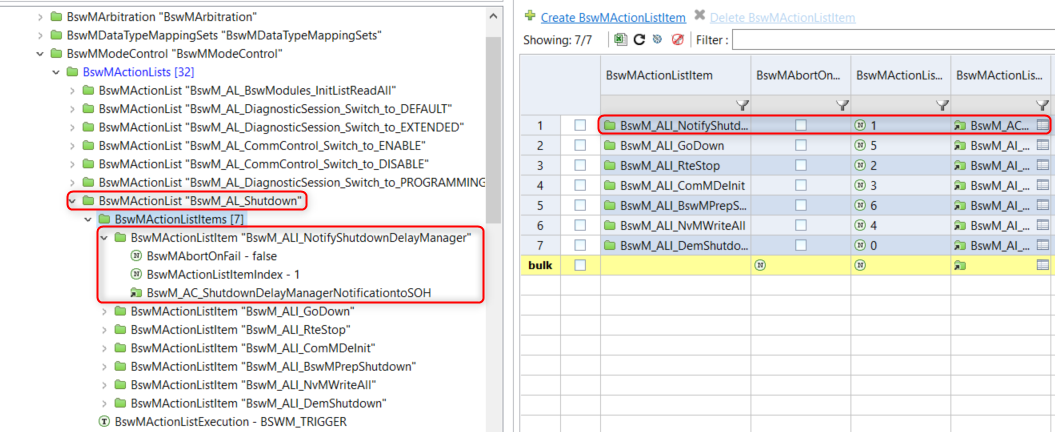
\includegraphics[scale=0.65]{images/shutdownconfiguration.png}
	\caption{Shutdown BswM action list sample}
	\label{fig:shutdownactionlist}
\end{figure}

The action list order is not striclty mandatory as in figure \ref{fig:shutdownactionlist}, but it is strongly suggested. 
\textbf{What is mandatory} for configuring the BSW in the right way, is that: \textit{The RteStop action \underline{must} come after than action that notifies the RTA-SUM SOH}; Otherwise
The callout will never be executed.
The RTA-SUM SOH notification action should be configured in a similar way to the following one:

\begin{figure}[h!]
	\centering
	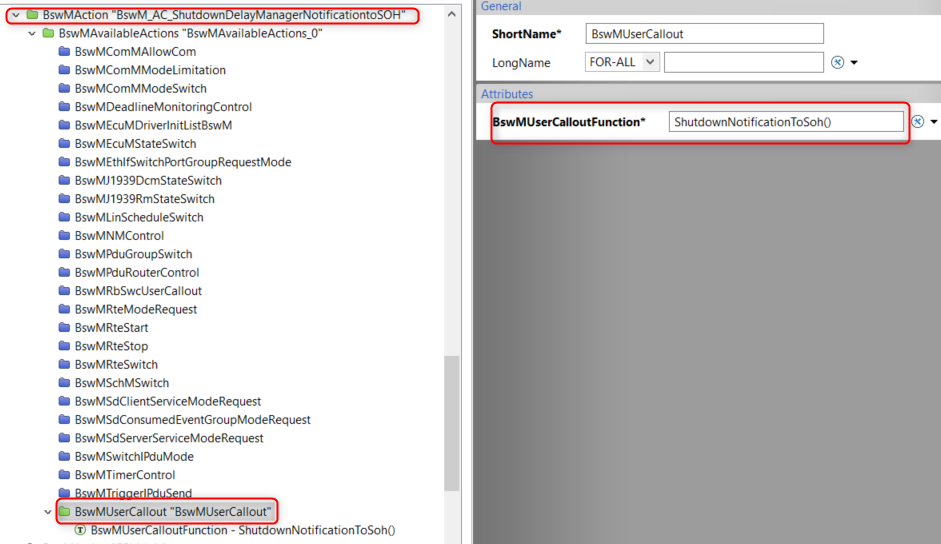
\includegraphics[scale=0.65]{images/calloutSohNot.png}
	\caption{Shutdown BswM action list sample}
	\label{fig:shutdownsohcallout}
\end{figure}

Once RTA-SUM SOH will receive this notification, it will disable the shutdown delay monitoring timer and it will take the current time from OS.
The value comparison will determine if the shutdown procedure has taken more time than allowed.\\
The delay monitoring timer can be blocked also by a wake-up occurrence during the shutdown delay monitoring (while timer still has not expired): if interfaces \code{SUSD_PermitExecution} or \\ \code{PNC_ShutdownPermission} do not 
match shutdown conditions anymore, the RTA-SUM SOH will disable AND reset the shutdown delay monitoring timer to the initial value, blocking the shutdown monitoring. In this case
no notification is expected from BSW.

\textbf{NOTE:} In case of
\begin{enumerate} 
	\item a continuous shutdown signals are being sent to RTA-SUM SOH
	\item RTA-SUM SOH Platform Reliability Monitor has already detected the request and it is working for monitoring the progresses
	\item Shutdown notification is never provided to RTA-SUM SOH (for any reason)
\end{enumerate}

The RTA-SUM SOH will count just only one failure in the Platform Reliability Monitor for the Shutdown delay monitoring. This means that
The RTA-SUM SOH will activate the Platform Reliability Monitor just when a change from normal execution request to a shutdown request is provided to it AND the shutdown notification OR wake-up request is provided to it during the shutdown delay monitoring.
\subsection{DID Counters}


\label{subsection:DIDCounters}
The user must configure the DcmDspData and DcmDspDidSignals properly in the DCM for each detector. An example is depicted in Figure \ref{fig:DID_F08F}.
\begin{figure}[H]
\centering
	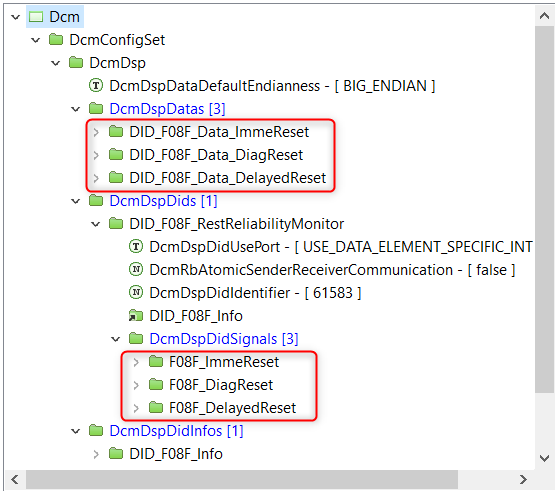
\includegraphics[scale=0.6]{images/DID_F08F}
	\caption{example of DID Configuration}
	\label{fig:DID_F08F}
\end{figure}

The NvM blocks and Dcm reference configuration must to be linked to the correct ones in the BSW for each detector. An example is depicted in Figure \ref{fig:DID_F092}.
\begin{figure}[H]
\centering
	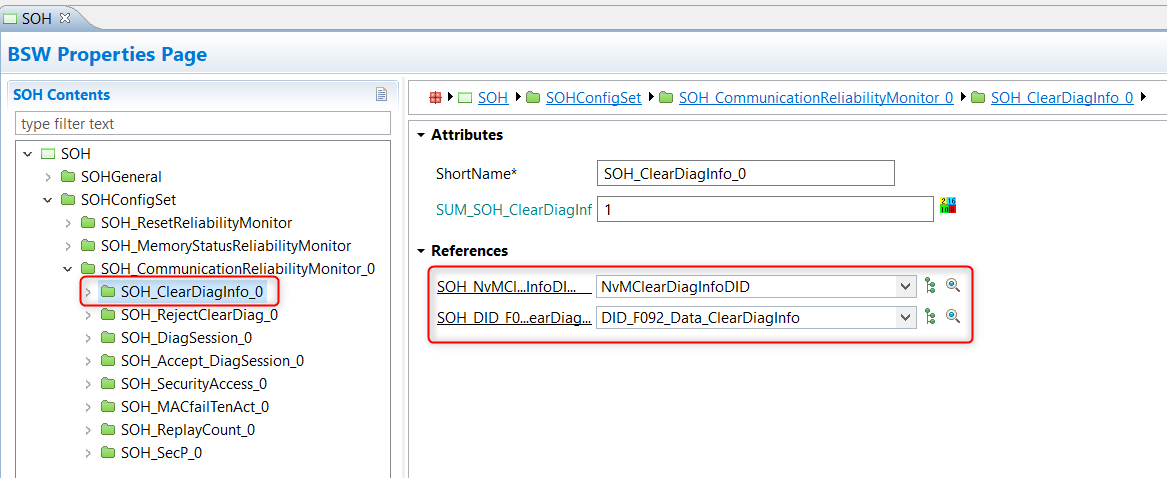
\includegraphics[scale=0.6]{images/DID_F092}
	\caption{example of reference configuration to BSW}
	\label{fig:DID_F092}
\end{figure}

To update the DID Counters values in the DCM you must schedule the following Runnables in an operation invoked event OS Task :

\begin{itemize}
	\item \code{Runnable_SOH_DID_F08F_Data_ImmeReset_Cntr} 
	\item \code{Runnable_SOH_DID_F08F_Data_DiagReset_Cntr} 
	\item \code{Runnable_SOH_DID_F08F_Data_DelayedReset_Cntr} 
	\item \code{Runnable_SOH_DID_F08F_CheckRead} 
	\item \code{Runnable_SOH_DID_F090_Data_StatNVM_Cntr}
	\item \code{Runnable_SOH_DID_F090_Data_ActNVM_Cntr}
	\item \code{Runnable_SOH_DID_F090_Data_PrivNVM_Cntr}
	\item \code{Runnable_SOH_DID_F090_Data_ExcepOS_Cntr}
	\item \code{Runnable_SOH_DID_F090_Data_ServOS_Cntr}
	\item \code{Runnable_SOH_DID_F090_Data_StackOS_Cntr}
	\item \code{Runnable_SOH_DID_F090_Data_MemProtOS_Cntr}
	\item \code{Runnable_SOH_DID_F090_Data_TimeProtOS_Cntr}
	\item \code{Runnable_SOH_DID_F090_Data_ErrOS_Cntr}
	\item \code{Runnable_SOH_DID_F090_CheckRead}
	\item \code{Runnable_SOH_DID_F091_Data_ShutDown_Cntr}
        \item \code{Runnable_SOH_DID_F091_CheckRead}
	\item \code{Runnable_SOH_DID_F092_Data_ClearDiagInfo_Cntr}
    \item \code{Runnable_SOH_DID_F092_Data_Reject_ClearDiag_Cntr}
    \item \code{Runnable_SOH_DID_F092_Data_DiagSession_Cntr}
    \item \code{Runnable_SOH_DID_F092_Data_Accept_DiagSession_Cntr}
    \item \code{Runnable_SOH_DID_F092_Data_SecurityAccess_Cntr}
    \item \code{Runnable_SOH_DID_F092_Data_MACfail_TenAct_Cntr}
    \item \code{Runnable_SOH_DID_F092_Data_ReplayCount_Cntr}
    \item \code{Runnable_SOH_DID_F092_Data_SecP_Cntr}
    \item \code{Runnable_SOH_DID_F092_CheckRead}
	\item \code{Runnable_SOH_DID_F093_Data_LocalStatFail_Cntr}
    \item \code{Runnable_SOH_DID_F093_Data_Data_WdgM_DEMErr_Cntr}
    \item \code{Runnable_SOH_DID_F093_Data_ERRHSupFail_Cntr}
    \item \code{Runnable_SOH_DID_F093_Data_ERRH_Local_Supervision_Status}
    \item \code{Runnable_SOH_DID_F093_CheckRead}

\end{itemize}

SUM\_SOH will populate the DIDs value in the BIG\_ENDIAN format. This is the expected endianness of the UDS layer.
Make sure to set DcmDspDataUsePort to CLIENT\_SERVER (means that the application, SUM\_SOH, is its manager). 

\subsection{WdgM}
\label{subsection:wdgm}
The SUM\_SOH releases for SDV 2.0 works as a Supervidsed Entity in order to be monitored by WdgM with an \textbf{Alive Supervision} method. This is possible thanks to Client-Server port \\ \textbf{RP\_SOH\_WdgM\_AliveSupervision}, with port interface \code{WdgM\_LocalSupervision}.
When Checkpoint is reached, SUM\_SOH sends a notification (the Alive Indication) to WdgM each time that \code{Runnable\_SOH\_} \\ \code{Main} is executed (Periodic Runnable).

The Alive Supervision requires the configuration of \textit{Supervsion Cycles} as time slots where the Alive Indication can be accepted for updating the Alive counting.

The duration of each Supervision Cycle represents the schedule time for \code{WdgM\_MainFunction} and it is configured thanks to parameters \code{WdgMSupervisionCycle} in WdgMConfigSet/WdgMMode.\\
Supervision Cycle length can be configured in order to occurr more frequently than Alive Indication or less, acording to own speicifc needs and AR specification about WdgM.

The configuration parameters to configure an Alive Supervision are represented in figure \ref{fig:as2}

\begin{figure}[h!]
	\centering
	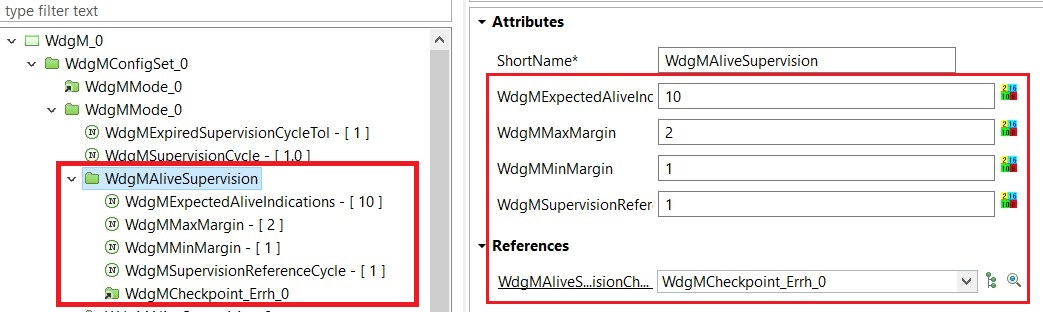
\includegraphics[scale=0.7]{images/wdgMAS}
	\caption{Configuration Parameters for Alive Supervision}
	\label{fig:as2}
\end{figure}

The configuration hints are the following:

\begin{itemize}
	\item \underline{\code{WdgMExpectedAliveIndications}}: This parameters shall contain the expected alive indication that can be derived from \code{WdgMSupervisionCycle} divided by \code{Runnable\_ERRH\_MainFunction} periodicity in addition to \code{WdgMSupervisionReferenceCycle};
	\item \underline{\code{WdgMMaxMargin}}: This parameters defines the number of extra Alive Indication that are tollerated;
	\item \underline{\code{WdgMMinMargin}}:  This parameters defines the number of less Alive Indication that are tollerated;
	\item \underline{\code{WdgMSupervisionReferenceCycle}}: This parameter is used to define the number of Supervision Cycles where the Alive Indications can arrive;
	\item \underline{\code{WdgMAliveSupervisionCheckpointRef}}: This is a reference to the Checkpoint that shall be reached to produce Alive Indication;
\end{itemize}

\subsection{RID 0x02C0 Clear SOH Logs}\label{sec:rid02c0}
To clear the SOH metrics the \code{Runnable_SOH_RIDClearLogs} is synchronicity invoked through an Operation Invoked Event in the DCM execution context.


It implements the Server part of the ClientServer Interface \code{RoutineServices_Clear_SUM_SOH_logs}. 

To obtain that interface you must configure, in the DCM container, a DcmDspRoutine named\newline
"Clear\_SUM\_SOH\_logs" that implements the RID 0x02C0 specifications described in the GB6001.

If at least one metric could not be written in the NvM due to an ongoing write activity or to an error during the NvM writing, the Routine will return a \code{DCM_E_GENERALREJECT} error code.

When the DCM calls the RID with an invalid Option Record values or an Option Record value related to a non-enabled detector/monitor, the Routine will return a \code{DCM_E_REQUESTOUTOFRANGE} error code.


The \textbf{Routine Status Record} is always set to the value \textbf{0x4} (Autosar supported, SOH integrated and RID executed). 
If the SUM\_SOH is not integrated in the system, the implementation of this routine and its status record value is in charge of the customer.

When the DCM calls the RID with Option Record values 0xF094 or 0xFFFF, the SUM\_SOH invokes a client operation service
in the SUM\_ERRH (Acting as a server) to clean all the metrics related to SUM\_SOH Local Supervision
Detector implemented at the ERRH side. To complete the RID 0x02C0 routine the SUM\_SOH shall interact
with the SUM\_ERRH through the Client-Server interface SOH\_ERRH \_RID\_Clear\_Logs where SUM\_ERRH
acts as a Server. 

Please connect the SUM\_SOH R-Port \textbf{RP\_SOH\_ERRH\_ClearRID0x02C0} with the relative one's of the SUM\_ERRH.

\subsection{RTE RteSwComponentType configuration}
\label{section:RteSwComponentType}
The component SUM\_SOH is delivered as source and not as object code. To configure in the right way the SUM\_SOH in your project, 
you need to create an \textbf{RteSwComponentType} that references the SUM\_SOH component and its SwcImplementation. 
Please check the Figure \ref{fig:as}

\begin{figure}[h!]
	\centering
	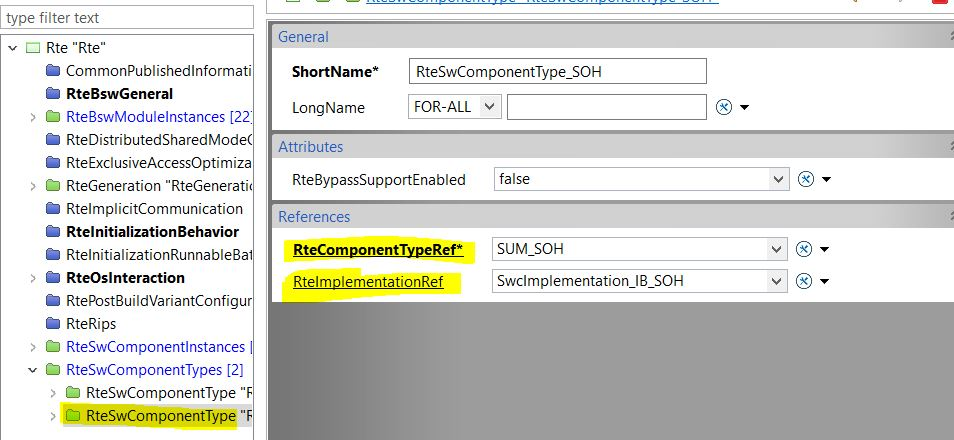
\includegraphics[scale=0.7]{images/RteSwComponentType}
	\caption{Configuration of RteSwComponentType}
	\label{fig:as}
\end{figure}